\chapter{実験1 : MNISTを用いた予備実験}

\section{概要}
本章では、本研究で提案するQuery-By-Dropout-Predictionsの有効性を検証するためにMNISTに対して行った実験について説明する。
Dropoutによってサンプリングされた各部分ネットワークの出力が未知データに対して分散を持つのかを検証し、
能動学習のクエリ選考基準として有効であるかを確認する。

\section{データセットについて}
MNISTは28×28ピクセルの手書き数字のデータセットである。
7万枚の画像からなり、そのうちの6万枚は訓練画像、残りの1万枚はテスト画像として利用される。
それぞれの画像は0~9までの数字ラベルが割り当てられているが、能動学習の状況を再現するため、
クエリとして問い合わせられるまではラベルへのアクセスが与えられない状況を設定する。

\section{実験設定}
\subsection{実験の詳細}

\begin{table}[h]
    \label{table:mnist_cnn}
    \caption{MNISTの実験に使用したCNNの構造を示す。}
    \center
    \begin{tabular}{|c|c|c|} \hline
        layer & size & activation \\ \hline
        Convolution & $32 \times 4 \times 4$ & relu \\
        Convolution & $32 \times 4 \times 4$ & relu \\
        Max Pooling & & \\
        dropout & & \\
        fully connected & 128 & relu \\
        dropout & & \\
        fully connected & 128 & relu \\
        \hline
    \end{tabular}
  \end{table}

識別器にはCNNを利用する。その構造を以下に示す\ref{table:mnist_cnn}(Kerasのexampleプログラムを参考にした)。
比較的小さなCNNであるため、クエリ問い合わせによってラベルが追加されるごとにfrom scratchからの再学習を行うことにする。
多層ニューラルネットワークの中では小さいモデルではあるものの、ラベルを一つずつ追加して再学習を行うのは計算コストが大きいため、バッチ型能動学習を採用する。
ここでも、同一クエリ内での情報の重複を避けるためクラスタリングを行う。
MNISTは784次元の画像で比較的小さいため、元の画像情報をそのまま特徴量としてk-meansによるクラスタリングを行う。
committeeサイズは20, k-meansのクラスター数$K$は100、一度に選択するクエリ$\mathcal{Q}$のサイズは10、再学習のepoch数は50に設定した。
また、クラスターの代表サンプルから無作為にサンプリングされた20個のサンプルをラベルを付与して学習初期のラベルつきデータとして実験を開始した。
各クエリ問い合わせ毎に10000枚のテストデータに対する識別精度を計測し、ラベルを付与されたデータが1000に到達するまで実験を続けた。
実験ごとのばらつきを考慮し、同一の実験を3回行いその平均と標準偏差を計算した。

\subsection{比較手法について}
提案するQuery-By-Dropout-Predictionsの性能を比較するため、いくつかの手法について実験を行った。
クエリの選考基準以外は全ての設定を揃えて実験を行った。

\subsubsection{提案手法}
推論時にDropoutを利用し、複数のpredictionを出力しそれらの平均の不確かさと不一致度を基準として利用する。
不確かさには予測分布のエントロピー(Entropy Sampling)を利用する。
\begin{eqnarray}
    score(x) =  -  \frac{1}{C} \sum_{c=i}^C KL \, (P_{\theta^{(c)}} || P_C) \, - \sum_i {P_C(y_i|x)} \log P_C(y|x)
\end{eqnarray}

\subsubsection{ナイーブなUncertainty Sampling}
推論時にDropoutを使用せずに単一の予測分布のエントロピーを利用する。
\begin{eqnarray}
    score(x) =  - \sum_i {P_{\theta}(y_i|x)} \log P_{\theta}(y|x)
\end{eqnarray}

\subsubsection{Dropoutにより周辺化した予測分布を利用したUncertainty Sampling}
推論時にDropoutを使用せずに単一の予測分布のエントロピーを利用する。\todo{このへんあやしいベイズCNNの話しないと}
\begin{eqnarray}
    score(x) =  - \sum_i {P_C(y_i|x)} \log P_C(y|x)
\end{eqnarray}

\subsubsection{Random Sampling}
この実験のベースラインと言える選択基準。各クエリ問い合わせ毎にランダムにサンプルを選択してラベル付きデータセットに追加する。

\section{実験結果}
本項では上記で述べた実験の結果を示す。
クエリ選考基準として提案手法、比較手法それぞれを使用した際の、ラベル付きサンプル数の増加に対するテスト精度の変化のグラフを図\ref{fig:mnist_acc_graph}に示す。
提案手法が僅かに性能が良いことが図からわかる。
また、\todo{引用}ならい、テストデータの識別精度が$90\%$、$95\%$を超えるのに要したラベルの数で比較する。
これでも良いことがわかる。
確かにUncertainly Samplingのみを用いた場合正しくモデル更新に寄与するサンプルを選択できていないことがわかる。
以下にラベル付きデータセットサイズが100の時にクエリとして選択されたサンプルを示す。図\ref{fig:mnist_query_sample}

\begin{figure}[tbp]
    \label{fig:mnist_acc_graph}
     \begin{center}
      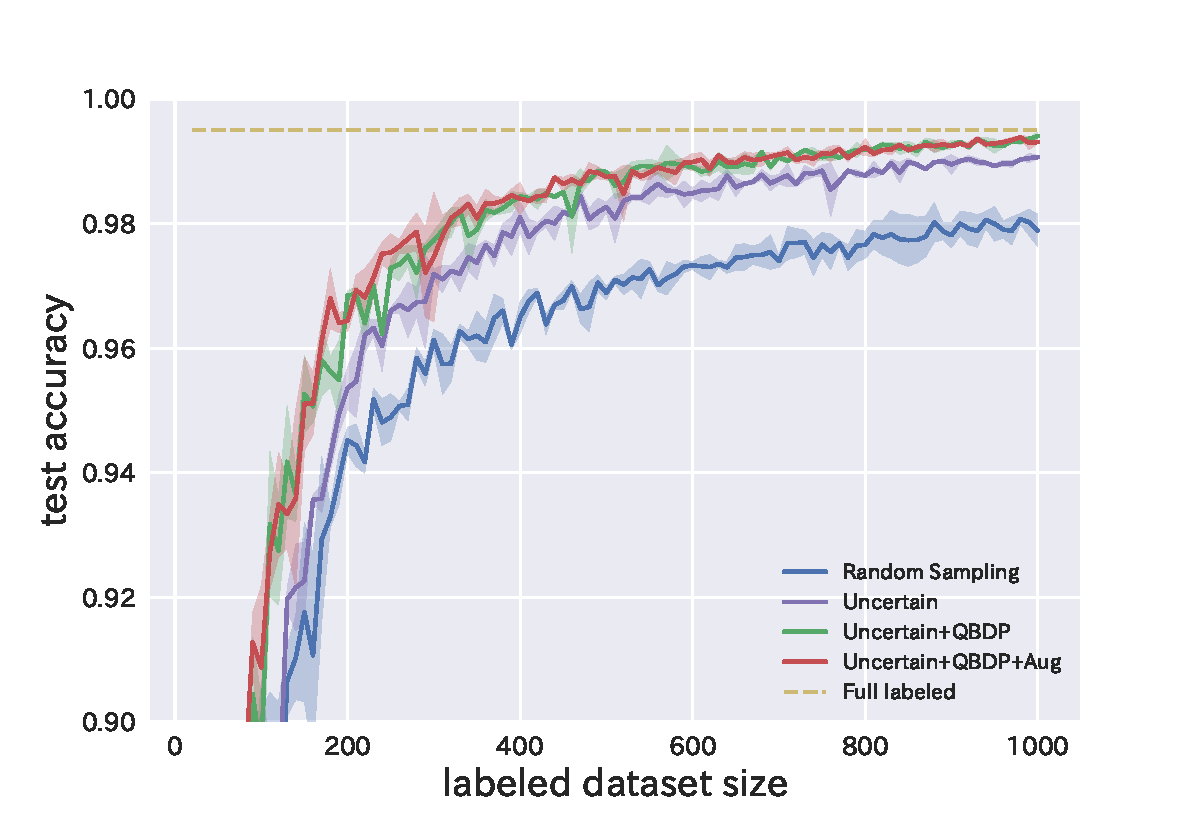
\includegraphics[width=10cm]{figures/mnist_acc_graph.pdf}
     \end{center}
    \caption{各手法を利用した場合のラベル付きサンプル数の増加に対するテスト精度の変化を示した図}
\end{figure}

\begin{table}[b]
    \label{table:mnist_samplenum_to_ccuracy}
    \caption{それぞれのクエリ選考基準を利用した場合にテスト精度を達成するために要したラベルの数}
    \center
    \begin{tabular}{c|c|c} 
        layer & $90\%$ & $95\%$ \\ \hline
        Proposed & 100 & 100 \\
        QBC only & 100 & 100 \\
        Uncertain Only & 100 & 100 \\
    \end{tabular}
\end{table}

\section{考察}
QBCがDeepと相性が良いことがわかった。
また、それを示すために訓練データとテストデータに対してDropoutを利用した場合のそれぞれの分布の分散を比較した。
